\chapter{Atomes et molécules}\label{ch:g7:atoms-and-molecules}

Prends une goutte d'eau et coupe-la en deux. Chaque moitié est encore
de l'eau. Coupe une moitié en deux, encore, et encore. Pourrait-on
continuer indéfiniment, ou finirait-on par obtenir un morceau si petit
que le couper une fois de plus donnerait quelque chose qui n'est plus du
tout de l'eau~? Vers 400~av.~J.-C., le penseur grec Démocrite a deviné
la réponse~: la matière est faite de minuscules morceaux que l'on ne
peut pas couper, qu'il a appelés \emph{\omterm{def:g7:atoms-and-molecules:atom}{atomes}}, du grec signifiant
«~insécable~». Il a fallu plus de deux mille ans, et le travail des
chimistes du \textsc{xix}\textsuperscript{e}~siècle, pour faire de
cette intuition une science. Ce chapitre décrit ces morceaux --- les
\omterm{def:g7:atoms-and-molecules:atom}{atomes} --- et la façon dont ils se regroupent en \omterm{def:g7:atoms-and-molecules:molecule}{molécules}.

\begin{recall}
Un \omterm{def:g6:pure-substances-and-mixtures:pure-substance}{corps pur}, comme l'eau ou le dioxygène, est constitué d'une seule
\omterm{def:g6:pure-substances-and-mixtures:species}{espèce chimique}~; un \omterm{def:g6:pure-substances-and-mixtures:mixture}{mélange}, comme l'\omterm{def:g4:air-a-mixture-of-gases:air}{air}, en contient plusieurs
(\cref{ch:g6:pure-substances-and-mixtures}). L'\omterm{def:g4:air-a-mixture-of-gases:air}{air} contient environ
quatre cinquièmes de diazote et un cinquième de dioxygène
(\cref{ch:g4:air-a-mixture-of-gases}).
\end{recall}

\section{Les atomes}

\begin{definition}[Atome]\label{def:g7:atoms-and-molecules:atom}
Toute la matière est construite à partir de particules extrêmement
petites appelées \emph{atomes}\index{atome}. Il n'existe dans la nature
qu'une centaine de sortes d'atomes différentes, et chaque substance ---
l'eau, l'\omterm{def:g4:air-a-mixture-of-gases:air}{air}, le fer, le sucre, notre propre corps --- est faite
d'atomes de quelques-unes de ces sortes.
\end{definition}

\begin{proposition}[Les atomes sont minuscules]\label{prop:g7:atoms-and-molecules:tiny}
% ledger: const:a0, earth:diameter (8 cm apple: 12756 km / 8 cm = 1.6 x 10^8;
% 0.1-0.15 nm x 1.6 x 10^8 = 1.7-2.4 cm, a small cherry)
Le plus petit \omterm{def:g7:atoms-and-molecules:atom}{atome}, l'\omterm{def:g7:atoms-and-molecules:atom}{atome} d'hydrogène, mesure environ un
dix-millionième de millimètre de diamètre~; les autres sont au plus
quelques fois plus gros. Dix millions d'\omterm{def:g7:atoms-and-molecules:atom}{atomes} d'hydrogène alignés
formeraient une ligne d'un millimètre. Pour se le représenter~: si une
pomme était agrandie jusqu'à la taille de la Terre, chacun de ses \omterm{def:g7:atoms-and-molecules:atom}{atomes}
aurait à peu près la taille d'une petite cerise.
\end{proposition}

\begin{remark}[Vus sans être vus]\label{rem:g7:atoms-and-molecules:seen}
Aucun microscope utilisant la lumière ne peut montrer un \omterm{def:g7:atoms-and-molecules:atom}{atome}~: les
\omterm{def:g7:atoms-and-molecules:atom}{atomes} sont bien plus petits que les ondes lumineuses. Depuis les années
1980, des microscopes spéciaux, qui palpent une surface avec une pointe
extrêmement fine, fournissent des images où les \omterm{def:g7:atoms-and-molecules:atom}{atomes} isolés
apparaissent comme des bosses.
\end{remark}

\begin{definition}[Symbole d'un atome]\label{def:g7:atoms-and-molecules:symbol}
Chaque sorte d'\omterm{def:g7:atoms-and-molecules:atom}{atome} a un nom et un \emph{symbole}\index{symbole d'un atome}~:
une lettre majuscule, parfois suivie d'une lettre minuscule. Le symbole
est le même dans toutes les langues.
\end{definition}

\begin{center}
\small
\begin{tabular}{llll|llll}
\hline
\omterm{def:g7:atoms-and-molecules:atom}{atome} & \omterm{def:g7:atoms-and-molecules:symbol}{symbole} & & couleur du modèle & \omterm{def:g7:atoms-and-molecules:atom}{atome} & \omterm{def:g7:atoms-and-molecules:symbol}{symbole} & & couleur du modèle \\
\hline
hydrogène & \ce{H} & \tikz\node[aH]{}; & blanc & sodium & \ce{Na} & \tikz\node[aNa]{}; & violet \\
carbone & \ce{C} & \tikz\node[aC]{}; & noir & soufre & \ce{S} & \tikz\node[aS]{}; & jaune \\
azote & \ce{N} & \tikz\node[aN]{}; & bleu & chlore & \ce{Cl} & \tikz\node[aCl]{}; & vert \\
oxygène & \ce{O} & \tikz\node[aO]{}; & rouge & fer, cuivre & \ce{Fe}, \ce{Cu} & & --- \\
\hline
\end{tabular}
\end{center}

\begin{remark}[D'où viennent les symboles]\label{rem:g7:atoms-and-molecules:latin}
La plupart des \omterm{def:g7:atoms-and-molecules:symbol}{symboles} sont les premières lettres du nom~: \ce{H} pour
l'hydrogène, \ce{C} pour le carbone, \ce{O} pour l'oxygène. Certains
viennent d'un nom latin plus ancien~: \ce{Na} pour le sodium
(\emph{natrium}), \ce{Fe} pour le fer (\emph{ferrum}), \ce{Cu} pour le
cuivre (\emph{cuprum}). La seconde lettre est toujours minuscule~:
\ce{Co} est l'\omterm{def:g7:atoms-and-molecules:atom}{atome} de cobalt, tandis que CO, avec un O majuscule, est
tout autre chose.
\end{remark}

\begin{history}[Les atomes de Dalton, 1808]
En 1808, le chimiste John Dalton publia un tableau des \omterm{def:g7:atoms-and-molecules:atom}{atomes} alors
connus, chacun dessiné comme un petit cercle portant son propre signe.
Il fut le premier à affirmer que tous les \omterm{def:g7:atoms-and-molecules:atom}{atomes} d'une même sorte ont le
même poids, et que les chimistes pouvaient comparer ces poids. Mais il
supposait aussi que l'eau était un \omterm{def:g7:atoms-and-molecules:atom}{atome} d'hydrogène lié à un \omterm{def:g7:atoms-and-molecules:atom}{atome}
d'oxygène~; il fallut encore cinquante ans pour que les chimistes
s'accordent sur le fait qu'une \omterm{def:g7:atoms-and-molecules:molecule}{molécule} d'eau contient \emph{deux}
\omterm{def:g7:atoms-and-molecules:atom}{atomes} d'hydrogène.
\end{history}

\begin{omfigure}
\begin{minipage}[b]{0.3\linewidth}\centering
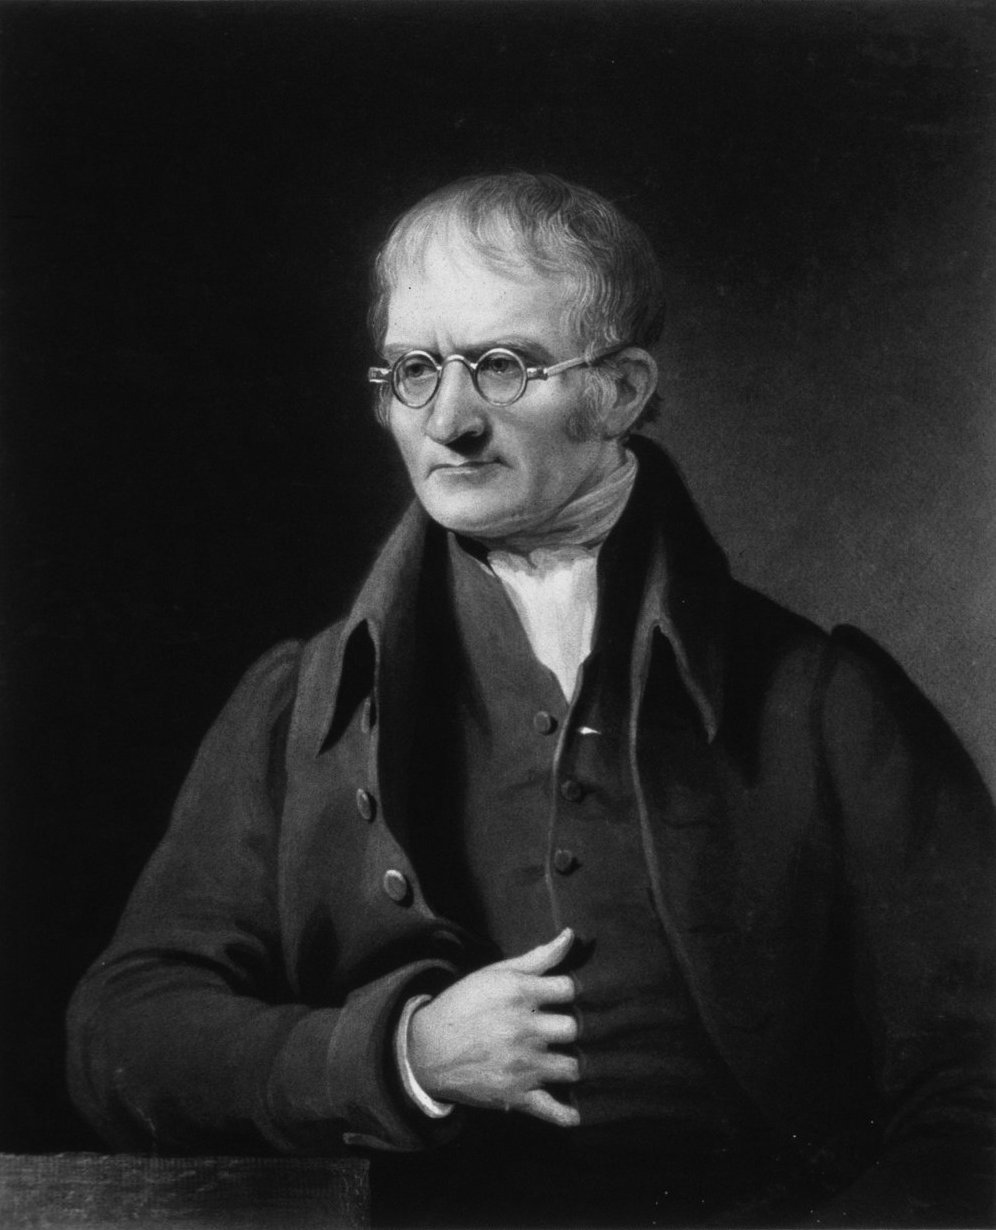
\includegraphics[width=\linewidth]{images/book1/dalton.jpg}

{\small John Dalton (1766--1844).}
\end{minipage}\hfill
\begin{minipage}[b]{0.66\linewidth}\centering
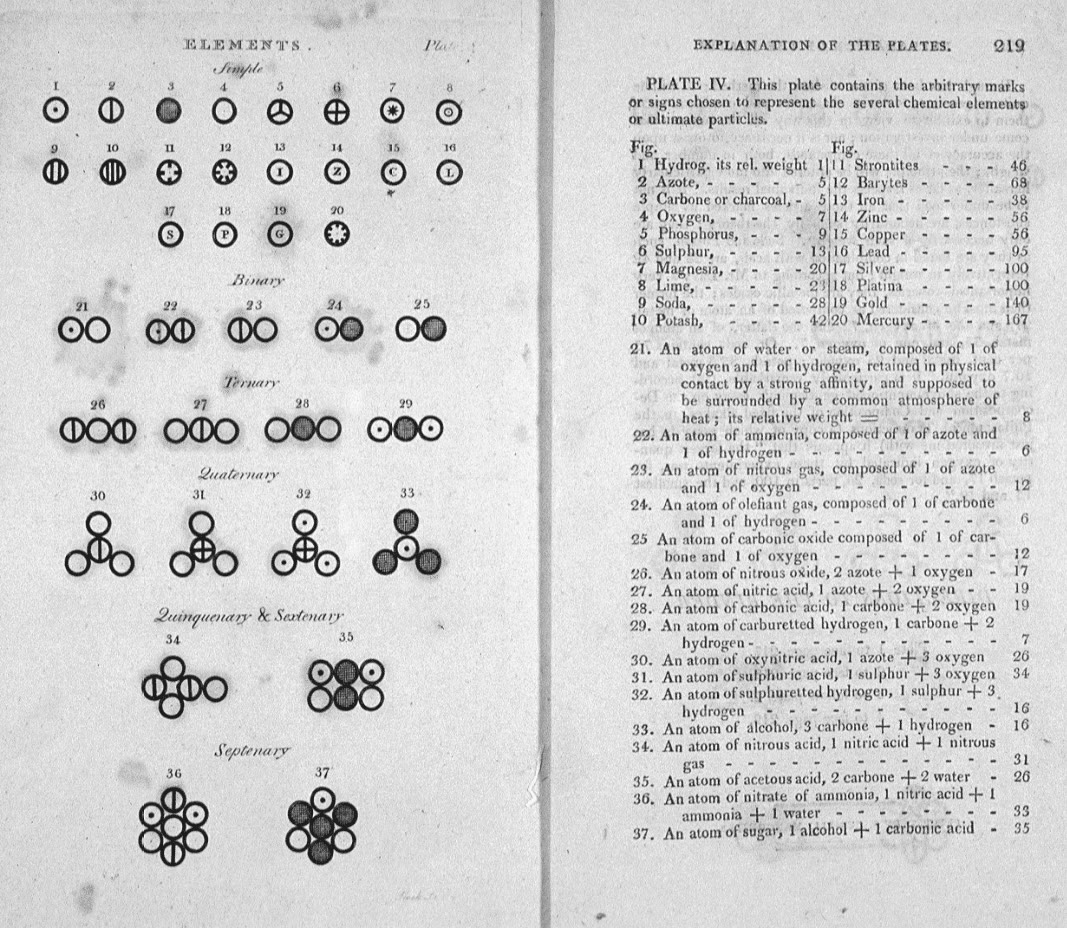
\includegraphics[width=\linewidth]{images/book1/dalton-symbols.jpg}

{\small Le tableau de Dalton de 1808~: son eau, le signe 21, est un
cercle d'hydrogène à côté d'un cercle d'oxygène.}
\end{minipage}
\end{omfigure}

\section{Les molécules}

\begin{definition}[Molécule]\label{def:g7:atoms-and-molecules:molecule}
Une \emph{molécule}\index{molecule@molécule} est un groupe d'\omterm{def:g7:atoms-and-molecules:atom}{atomes} solidement
liés entre eux. Une molécule est le plus petit morceau d'une substance
qui soit encore cette substance~: une molécule d'eau est la plus petite
quantité d'eau possible.
\end{definition}

\begin{example}[Sept molécules]\label{ex:g7:atoms-and-molecules:seven}
\begin{itemize}
  \item la \omterm{def:g7:atoms-and-molecules:molecule}{molécule} de \emph{dihydrogène}~: deux \omterm{def:g7:atoms-and-molecules:atom}{atomes} d'hydrogène~;
  \item la \omterm{def:g7:atoms-and-molecules:molecule}{molécule} de \emph{dioxygène}, que nous respirons~: deux
        \omterm{def:g7:atoms-and-molecules:atom}{atomes} d'oxygène~;
  \item la \omterm{def:g7:atoms-and-molecules:molecule}{molécule} de \emph{diazote}, les quatre cinquièmes de l'\omterm{def:g4:air-a-mixture-of-gases:air}{air}~:
        deux \omterm{def:g7:atoms-and-molecules:atom}{atomes} d'azote~;
  \item la \omterm{def:g7:atoms-and-molecules:molecule}{molécule} d'\emph{eau}~: deux \omterm{def:g7:atoms-and-molecules:atom}{atomes} d'hydrogène et un \omterm{def:g7:atoms-and-molecules:atom}{atome}
        d'oxygène~;
  \item la \omterm{def:g7:atoms-and-molecules:molecule}{molécule} de \emph{dioxyde de carbone}, que nous expirons~: un
        \omterm{def:g7:atoms-and-molecules:atom}{atome} de carbone et deux \omterm{def:g7:atoms-and-molecules:atom}{atomes} d'oxygène~;
  \item la \omterm{def:g7:atoms-and-molecules:molecule}{molécule} de \emph{méthane}, le principal constituant du gaz
        naturel brûlé dans les cuisinières~: un \omterm{def:g7:atoms-and-molecules:atom}{atome} de carbone et quatre
        \omterm{def:g7:atoms-and-molecules:atom}{atomes} d'hydrogène~;
  \item la \omterm{def:g7:atoms-and-molecules:molecule}{molécule} de \emph{protoxyde d'azote}, un gaz anesthésiant~:
        deux \omterm{def:g7:atoms-and-molecules:atom}{atomes} d'azote et un \omterm{def:g7:atoms-and-molecules:atom}{atome} d'oxygène.
\end{itemize}
\end{example}

\begin{omfigure}
\begin{tikzpicture}[font=\small]
  % hydrogen
  \begin{scope}[xshift=0cm]
    \node[aH] (a) at (-0.25,0) {}; \node[aH] (b) at (0.25,0) {};
    \begin{scope}[on background layer]\draw[bond] (a.center) -- (b.center);\end{scope}
    \node at (0,-1.05) {dihydrogène};
  \end{scope}
  % oxygen
  \begin{scope}[xshift=2.6cm]
    \node[aO] (a) at (-0.33,0) {}; \node[aO] (b) at (0.33,0) {};
    \begin{scope}[on background layer]
      \draw[bond, line width=1.1pt] ([yshift=1.6pt]a.center) -- ([yshift=1.6pt]b.center);
      \draw[bond, line width=1.1pt] ([yshift=-1.6pt]a.center) -- ([yshift=-1.6pt]b.center);
    \end{scope}
    \node at (0,-1.05) {dioxygène};
  \end{scope}
  % nitrogen
  \begin{scope}[xshift=5.2cm]
    \node[aN] (a) at (-0.33,0) {}; \node[aN] (b) at (0.33,0) {};
    \begin{scope}[on background layer]
      \foreach \d in {-2.4,0,2.4}
        \draw[bond, line width=0.9pt] ([yshift=\d pt]a.center) -- ([yshift=\d pt]b.center);
    \end{scope}
    \node at (0,-1.05) {diazote};
  \end{scope}
  % water
  \begin{scope}[xshift=7.8cm, yshift=0.2cm]
    \node[aO] (o) at (0,0) {};
    \node[aH] (h1) at (-0.62,-0.48) {}; \node[aH] (h2) at (0.62,-0.48) {};
    \begin{scope}[on background layer]
      \draw[bond] (o.center) -- (h1.center); \draw[bond] (o.center) -- (h2.center);
    \end{scope}
    \node at (0,-1.25) {eau};
  \end{scope}
  % carbon dioxide
  \begin{scope}[xshift=0.9cm, yshift=-2.7cm]
    \node[aO] (a) at (-0.85,0) {}; \node[aC] (c) at (0,0) {}; \node[aO] (b) at (0.85,0) {};
    \begin{scope}[on background layer]
      \foreach \d in {-1.6,1.6} {
        \draw[bond, line width=1.1pt] ([yshift=\d pt]a.center) -- ([yshift=\d pt]c.center);
        \draw[bond, line width=1.1pt] ([yshift=\d pt]c.center) -- ([yshift=\d pt]b.center);}
    \end{scope}
    \node at (0,-1.05) {dioxyde de carbone};
  \end{scope}
  % methane
  \begin{scope}[xshift=4.4cm, yshift=-2.6cm]
    \node[aC] (c) at (0,0) {};
    \node[aH] (h1) at (0,0.78) {};
    \node[aH] (h2) at (-0.74,-0.3) {};
    \node[aH] (h3) at (0.74,-0.3) {};
    \begin{scope}[on background layer]
      \draw[bond] (c.center) -- (h1.center); \draw[bond] (c.center) -- (h2.center);
      \draw[bond] (c.center) -- (h3.center);
    \end{scope}
    \draw[bond] (c.center) -- (0.22,-0.52);
    \node[aH] at (0.24,-0.58) {};
    \node at (0,-1.15) {méthane};
  \end{scope}
  % nitrous oxide
  \begin{scope}[xshift=7.8cm, yshift=-2.7cm]
    \node[aN] (a) at (-0.8,0) {}; \node[aN] (b) at (0,0) {}; \node[aO] (c) at (0.8,0) {};
    \begin{scope}[on background layer]
      \foreach \d in {-1.6,1.6} {
        \draw[bond, line width=1.1pt] ([yshift=\d pt]a.center) -- ([yshift=\d pt]b.center);
        \draw[bond, line width=1.1pt] ([yshift=\d pt]b.center) -- ([yshift=\d pt]c.center);}
    \end{scope}
    \node at (0,-1.05) {protoxyde d'azote};
  \end{scope}
\end{tikzpicture}

{\small Modèles moléculaires éclatés des sept \omterm{def:g7:atoms-and-molecules:molecule}{molécules} de
l'\cref{ex:g7:atoms-and-molecules:seven}. Chaque bâtonnet représente une
liaison entre deux \omterm{def:g7:atoms-and-molecules:atom}{atomes}~; pourquoi certains \omterm{def:g7:atoms-and-molecules:atom}{atomes} partagent deux ou
trois bâtonnets est expliqué dans un chapitre suivant.}
\end{omfigure}

\begin{proposition}[Les molécules d'un corps pur et d'un mélange]\label{prop:g7:atoms-and-molecules:pure}
Dans un \omterm{def:g6:pure-substances-and-mixtures:pure-substance}{corps pur} constitué de \omterm{def:g7:atoms-and-molecules:molecule}{molécules}, toutes les \omterm{def:g7:atoms-and-molecules:molecule}{molécules} sont
identiques~: l'eau pure ne contient que des \omterm{def:g7:atoms-and-molecules:molecule}{molécules} d'eau. Un \omterm{def:g6:pure-substances-and-mixtures:mixture}{mélange}
contient des \omterm{def:g7:atoms-and-molecules:molecule}{molécules} de plusieurs sortes~: l'\omterm{def:g4:air-a-mixture-of-gases:air}{air} est surtout fait de
\omterm{def:g7:atoms-and-molecules:molecule}{molécules} de diazote et de \omterm{def:g7:atoms-and-molecules:molecule}{molécules} de dioxygène, environ quatre de
diazote pour une de dioxygène, avec quelques \omterm{def:g7:atoms-and-molecules:atom}{atomes} d'argon qui restent
isolés, et très peu de \omterm{def:g7:atoms-and-molecules:molecule}{molécules} de dioxyde de carbone.
\end{proposition}

\begin{omfigure}
\begin{tikzpicture}[font=\small,
    sN/.style={aN, minimum size=3.0mm}, sO/.style={aO, minimum size=2.9mm},
    sH/.style={aH, minimum size=2.1mm}, sAr/.style={om atom, ball color=cyan!60, minimum size=3.4mm}]
  % air
  \draw[omGlass, line width=0.6pt] (0,0) rectangle (3.4,3.4);
  \foreach \x/\y/\r in {0.5/0.6/20, 1.6/0.4/-30, 2.8/0.7/75, 0.6/1.7/110,
                        2.0/1.5/10, 2.9/2.0/-60, 0.9/2.8/40, 2.1/2.9/-15}
    \node[sN] at ($(\x,\y)+(\r:0.12)$) {} node[sN] at ($(\x,\y)+(\r+180:0.12)$) {};
  \foreach \x/\y/\r in {1.3/1.1/60, 1.6/2.3/-40}
    \node[sO] at ($(\x,\y)+(\r:0.12)$) {} node[sO] at ($(\x,\y)+(\r+180:0.12)$) {};
  \node[sAr] at (2.9,3.0) {};
  \node[anchor=north] at (1.7,-0.1) {\textbf{air}~: un mélange};
  % water
  \begin{scope}[xshift=5.2cm]
    \draw[omGlass, line width=0.6pt] (0,0) rectangle (3.4,3.4);
    \foreach \x in {0,1,2,3,4} \foreach \y in {0,1,2,3,4} {
      \pgfmathsetmacro{\ang}{mod(73*\x+41*\y,360)}
      \begin{scope}[shift={({0.36+0.67*\x},{0.4+0.66*\y})}, rotate=\ang]
        \node[sH] at (-0.16,-0.12) {}; \node[sH] at (0.16,-0.12) {};
        \node[sO] at (0,0) {};
      \end{scope}}
    \node[anchor=north] at (1.7,-0.1) {\textbf{eau}~: un corps pur};
  \end{scope}
\end{tikzpicture}

{\small Un zoom énorme. À gauche~: dans l'\omterm{def:g4:air-a-mixture-of-gases:air}{air}, les \omterm{def:g7:atoms-and-molecules:molecule}{molécules} de diazote
(bleues) sont bien plus nombreuses que celles de dioxygène (rouges), et
un \omterm{def:g7:atoms-and-molecules:atom}{atome} d'argon (bleu pâle) voyage seul~; les \omterm{def:g7:atoms-and-molecules:molecule}{molécules} d'un gaz sont
très éloignées les unes des autres. À droite~: dans l'eau liquide, les
\omterm{def:g7:atoms-and-molecules:molecule}{molécules} sont toutes identiques et se touchent.}
\end{omfigure}

\section{Les formules chimiques}

\begin{definition}[Formule chimique]\label{def:g7:atoms-and-molecules:formula}
La \emph{formule chimique}\index{formule chimique} d'une \omterm{def:g7:atoms-and-molecules:molecule}{molécule}
énumère les \omterm{def:g7:atoms-and-molecules:symbol}{symboles} de ses \omterm{def:g7:atoms-and-molecules:atom}{atomes}, chacun suivi d'un petit nombre écrit
en bas à droite --- l'\emph{indice}\index{indice} --- qui donne le
nombre d'\omterm{def:g7:atoms-and-molecules:atom}{atomes} de cette sorte que contient la \omterm{def:g7:atoms-and-molecules:molecule}{molécule}. Un indice 1 ne
s'écrit pas.
\end{definition}

\begin{example}[Les sept formules]\label{ex:g7:atoms-and-molecules:formulas}
Les \omterm{def:g7:atoms-and-molecules:molecule}{molécules} de l'\cref{ex:g7:atoms-and-molecules:seven} ont pour
formules~:
\begin{center}
\begin{tabular}{lcl}
\hline
\omterm{def:g7:atoms-and-molecules:molecule}{molécule} & formule & \omterm{def:g7:atoms-and-molecules:atom}{atomes} \\
\hline
dihydrogène & \ce{H2} & 2 hydrogènes \\
dioxygène & \ce{O2} & 2 oxygènes \\
diazote & \ce{N2} & 2 azotes \\
eau & \ce{H2O} & 2 hydrogènes, 1 oxygène \\
dioxyde de carbone & \ce{CO2} & 1 carbone, 2 oxygènes \\
méthane & \ce{CH4} & 1 carbone, 4 hydrogènes \\
protoxyde d'azote & \ce{N2O} & 2 azotes, 1 oxygène \\
\hline
\end{tabular}
\end{center}
\end{example}

\begin{method}[Lire une formule]\label{met:g7:atoms-and-molecules:read}
Pour lire la formule d'une \omterm{def:g7:atoms-and-molecules:molecule}{molécule}~:
\begin{enumerate}
  \item la découper en \omterm{def:g7:atoms-and-molecules:symbol}{symboles}~: chacun commence par une majuscule~;
  \item après chaque \omterm{def:g7:atoms-and-molecules:symbol}{symbole}, lire l'\omterm{def:g7:atoms-and-molecules:formula}{indice} (pas d'\omterm{def:g7:atoms-and-molecules:formula}{indice} veut dire 1)~;
  \item additionner les \omterm{def:g7:atoms-and-molecules:formula}{indices} pour obtenir le nombre total d'\omterm{def:g7:atoms-and-molecules:atom}{atomes}.
\end{enumerate}
Pour \ce{C2H6O} (l'éthanol, l'alcool des boissons)~: 2 carbones,
6 hydrogènes, 1 oxygène, soit 9 \omterm{def:g7:atoms-and-molecules:atom}{atomes} en tout.
\end{method}

\begin{remark}[Un nombre devant]\label{rem:g7:atoms-and-molecules:coefficient}
Un nombre écrit devant une formule compte des \omterm{def:g7:atoms-and-molecules:molecule}{molécules}~: \ce{3H2O}
désigne trois \omterm{def:g7:atoms-and-molecules:molecule}{molécules} d'eau, qui contiennent ensemble 6 \omterm{def:g7:atoms-and-molecules:atom}{atomes}
d'hydrogène et 3 \omterm{def:g7:atoms-and-molecules:atom}{atomes} d'oxygène. Il ne faut pas confondre \ce{O2}, une
\omterm{def:g7:atoms-and-molecules:molecule}{molécule} formée de deux \omterm{def:g7:atoms-and-molecules:atom}{atomes} d'oxygène, avec \ce{2O}, deux \omterm{def:g7:atoms-and-molecules:atom}{atomes}
d'oxygène qui ne sont pas liés.
\end{remark}

\begin{example}[Le méthane dans la cuisine]\label{ex:g7:atoms-and-molecules:methane}
Le gaz naturel d'une cuisinière est surtout du méthane, \ce{CH4}.
Chacune de ses \omterm{def:g7:atoms-and-molecules:molecule}{molécules} est un \omterm{def:g7:atoms-and-molecules:atom}{atome} de carbone entouré de quatre
\omterm{def:g7:atoms-and-molecules:atom}{atomes} d'hydrogène. Ce gaz est invisible et n'a pas d'odeur~: l'odeur
du «~gaz~» est celle d'une substance ajoutée exprès, pour qu'une fuite
se remarque.
\end{example}

\begin{omfigure}
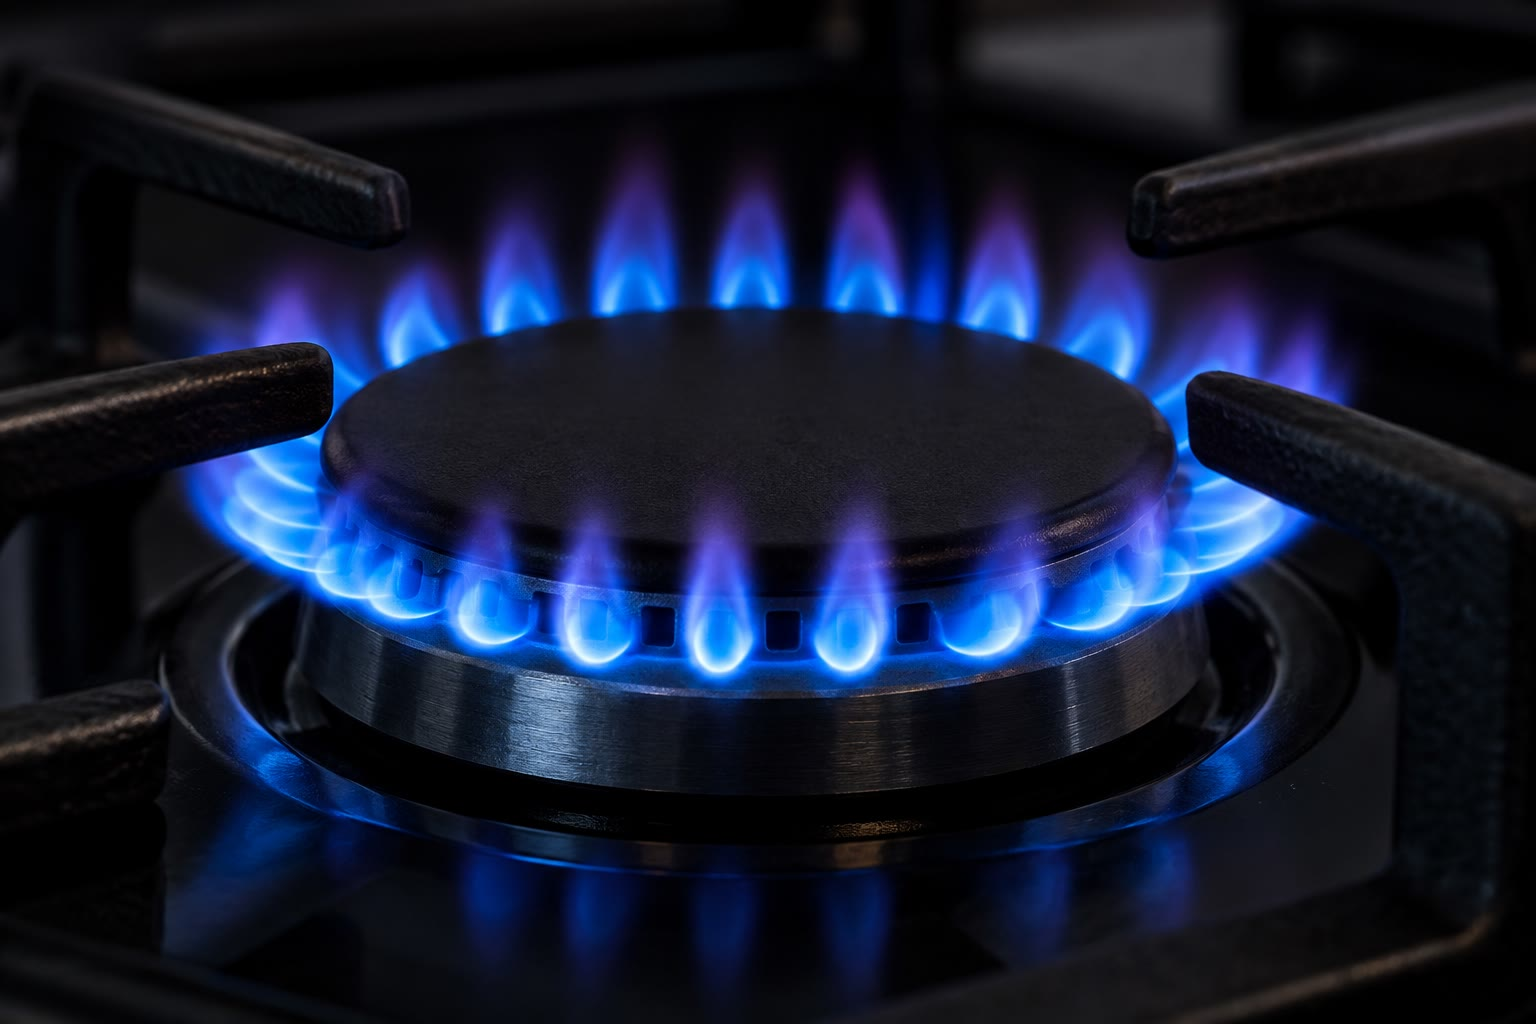
\includegraphics[width=0.5\linewidth]{images/book1/ai/g7-gas-flame.jpg}

{\small La flamme bleue d'une cuisinière à gaz~: le méthane du gaz
naturel \omterm{def:g4:what-a-fire-needs:burning}{brûle}.}
\end{omfigure}

\section{Les modèles moléculaires}

\begin{remark}[Les modèles et leurs couleurs]\label{rem:g7:atoms-and-molecules:models}
Les chimistes construisent des \emph{modèles moléculaires} avec des
boules pour les \omterm{def:g7:atoms-and-molecules:atom}{atomes} et des bâtonnets pour les liaisons entre eux. Les
couleurs sont une convention utilisée dans le monde entier --- carbone
noir, hydrogène blanc, oxygène rouge, azote bleu --- et non la vraie
couleur des \omterm{def:g7:atoms-and-molecules:atom}{atomes}~: un \omterm{def:g7:atoms-and-molecules:atom}{atome} isolé n'a aucune couleur. Un modèle montre
aussi la forme d'une \omterm{def:g7:atoms-and-molecules:molecule}{molécule}, ce que ne fait pas une formule~: la
\omterm{def:g7:atoms-and-molecules:molecule}{molécule} d'eau est coudée, la \omterm{def:g7:atoms-and-molecules:molecule}{molécule} de dioxyde de carbone est
linéaire.
\end{remark}

\begin{omfigure}
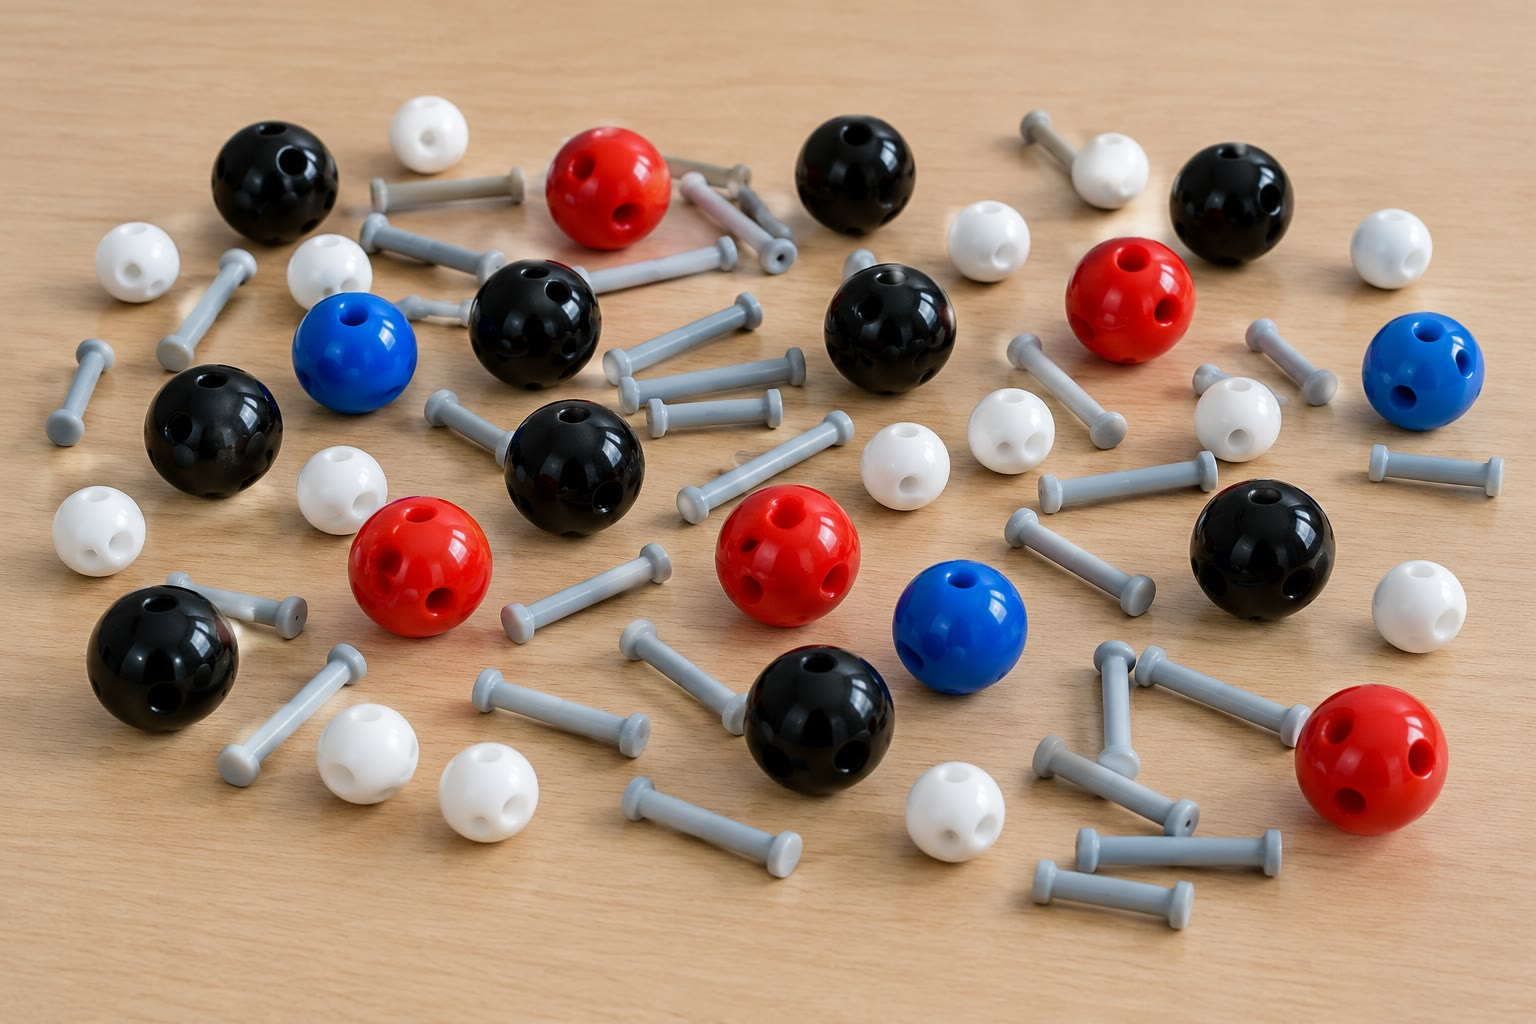
\includegraphics[width=0.5\linewidth]{images/book1/ai/g7-model-kit.jpg}

{\small Une boîte de modèles moléculaires~: des boules pour les \omterm{def:g7:atoms-and-molecules:atom}{atomes},
percées de trous pour les bâtonnets qui représentent les liaisons.}
\end{omfigure}

\begin{method}[D'un modèle à une formule]\label{met:g7:atoms-and-molecules:model}
Pour écrire la formule d'une \omterm{def:g7:atoms-and-molecules:molecule}{molécule} à partir de son modèle~:
\begin{enumerate}
  \item nommer les \omterm{def:g7:atoms-and-molecules:atom}{atomes} d'après leurs couleurs~;
  \item compter les boules de chaque couleur~;
  \item écrire les \omterm{def:g7:atoms-and-molecules:symbol}{symboles} avec les nombres en \omterm{def:g7:atoms-and-molecules:formula}{indice}, le carbone
        d'abord, puis l'hydrogène, puis les autres \omterm{def:g7:atoms-and-molecules:atom}{atomes} dans l'ordre
        alphabétique de leurs \omterm{def:g7:atoms-and-molecules:symbol}{symboles}.
\end{enumerate}
Une boule noire liée à quatre boules blanches~: un carbone, quatre
hydrogènes, \ce{CH4}.
\end{method}

\section{Exercices}

\begin{exercise}[$\star$]\label{exo:g7:atoms-and-molecules:1}
Qu'est-ce qu'un \omterm{def:g7:atoms-and-molecules:atom}{atome}~? Qu'est-ce qu'une \omterm{def:g7:atoms-and-molecules:molecule}{molécule}~?
\end{exercise}

\begin{exercise}[$\star$]\label{exo:g7:atoms-and-molecules:2}
Donne les \omterm{def:g7:atoms-and-molecules:symbol}{symboles} de l'hydrogène, du carbone, de l'azote, de
l'oxygène, du sodium et du fer.
\end{exercise}

\begin{exercise}[$\star$]\label{exo:g7:atoms-and-molecules:3}
Combien d'\omterm{def:g7:atoms-and-molecules:atom}{atomes} de chaque sorte y a-t-il dans une \omterm{def:g7:atoms-and-molecules:molecule}{molécule} de dioxyde
de carbone, \ce{CO2}~? Combien d'\omterm{def:g7:atoms-and-molecules:atom}{atomes} en tout~?
\end{exercise}

\begin{exercise}[$\star$]\label{exo:g7:atoms-and-molecules:4}
Nomme les \omterm{def:g7:atoms-and-molecules:molecule}{molécules} \ce{H2O}, \ce{O2}, \ce{CH4} et \ce{N2}.
\end{exercise}

\begin{exercise}[$\star$]\label{exo:g7:atoms-and-molecules:5}
Une \omterm{def:g7:atoms-and-molecules:molecule}{molécule} de dioxyde d'azote, un gaz brun présent dans l'\omterm{def:g4:air-a-mixture-of-gases:air}{air} pollué,
est formée d'un \omterm{def:g7:atoms-and-molecules:atom}{atome} d'azote et de deux \omterm{def:g7:atoms-and-molecules:atom}{atomes} d'oxygène. Écris sa
formule.
\end{exercise}

\begin{exercise}[$\star\star$]\label{exo:g7:atoms-and-molecules:6}
Explique la différence entre \ce{O2} et \ce{2O}, et entre \ce{CO} et
\ce{Co}.
\end{exercise}

\begin{exercise}[$\star\star$]\label{exo:g7:atoms-and-molecules:7}
Combien d'\omterm{def:g7:atoms-and-molecules:atom}{atomes} d'hydrogène et combien d'\omterm{def:g7:atoms-and-molecules:atom}{atomes} d'oxygène y a-t-il dans
\ce{3H2O}~? Dans \ce{5O2}~?
\end{exercise}

\begin{exercise}[$\star\star$]\label{exo:g7:atoms-and-molecules:8}
Un modèle est formé d'une boule noire liée à deux boules rouges. Nomme
les \omterm{def:g7:atoms-and-molecules:atom}{atomes}, écris la formule et nomme la \omterm{def:g7:atoms-and-molecules:molecule}{molécule}.
\end{exercise}

\begin{exercise}[$\star\star$]\label{exo:g7:atoms-and-molecules:9}
Dans le tableau de Dalton, l'eau est formée d'un \omterm{def:g7:atoms-and-molecules:atom}{atome} d'hydrogène et
d'un \omterm{def:g7:atoms-and-molecules:atom}{atome} d'oxygène. Écris la formule que Dalton avait en tête, et dis
combien d'\omterm{def:g7:atoms-and-molecules:atom}{atomes} il manque à sa \omterm{def:g7:atoms-and-molecules:molecule}{molécule} d'eau.
\end{exercise}

\begin{exercise}[$\star\star$]\label{exo:g7:atoms-and-molecules:10}
L'eau pure est-elle un \omterm{def:g6:pure-substances-and-mixtures:mixture}{mélange}~? Et l'\omterm{def:g4:air-a-mixture-of-gases:air}{air}~? Réponds en décrivant les
\omterm{def:g7:atoms-and-molecules:molecule}{molécules} que chacun contient.
\end{exercise}

\begin{exercise}[$\star\star\star$]\label{exo:g7:atoms-and-molecules:11}
Un \omterm{def:g7:atoms-and-molecules:atom}{atome} d'hydrogène mesure environ un dix-millionième de millimètre de
diamètre. Combien d'\omterm{def:g7:atoms-and-molecules:atom}{atomes} d'hydrogène, côte à côte, formeraient une
ligne de \qty{1}{cm}~? Et une ligne aussi longue qu'un terrain de
football, \qty{100}{m}~?
\end{exercise}

\begin{exercise}[$\star\star\star$]\label{exo:g7:atoms-and-molecules:12}
Le glucose, le sucre qui nourrit nos cellules, a pour formule
\ce{C6H12O6}. Combien d'\omterm{def:g7:atoms-and-molecules:atom}{atomes} une \omterm{def:g7:atoms-and-molecules:molecule}{molécule} de glucose contient-elle~?
Quel pourcentage d'entre eux sont des \omterm{def:g7:atoms-and-molecules:atom}{atomes} d'hydrogène~? Quel
pourcentage sont des \omterm{def:g7:atoms-and-molecules:atom}{atomes} de carbone~?
\end{exercise}

\section{Problème~: les atomes d'un souffle}

\begin{problem}[{Problème du week-end --- compter les atomes d'une
bouffée d'air, avant et après son passage dans nos poumons}]
\label{pb:g7:atoms-and-molecules:1}
% ledger: air:N2, air:O2, air:Ar (78.08 / 20.95 / 0.93 rounded to 78 / 21 / 1),
% breath:O2, breath:CO2, breath:N2 (expired air: 16 / 4 / 78, water vapour removed)
Le diazote traverse les poumons sans changer~: il fait donc un bon étalon.
Dans l'\omterm{def:g4:air-a-mixture-of-gases:air}{air} sec, pour 78 \omterm{def:g7:atoms-and-molecules:molecule}{molécules} de diazote, il y a environ 21 \omterm{def:g7:atoms-and-molecules:molecule}{molécules}
de dioxygène et 1 \omterm{def:g7:atoms-and-molecules:atom}{atome} d'argon~: 100 particules (\omterm{def:g7:atoms-and-molecules:molecule}{molécules} ou \omterm{def:g7:atoms-and-molecules:atom}{atomes}
isolés) en tout. Dans l'\omterm{def:g4:air-a-mixture-of-gases:air}{air} expiré, une fois sa vapeur d'eau retirée, les
mêmes 78 \omterm{def:g7:atoms-and-molecules:molecule}{molécules} de diazote sont accompagnées d'environ 16 \omterm{def:g7:atoms-and-molecules:molecule}{molécules} de
dioxygène, 4 \omterm{def:g7:atoms-and-molecules:molecule}{molécules} de dioxyde de carbone et 1 \omterm{def:g7:atoms-and-molecules:atom}{atome} d'argon.

\medskip
\noindent\textbf{Partie I --- L'\omterm{def:g4:air-a-mixture-of-gases:air}{air} que nous inspirons.}
\begin{enumerate}
  \item Écris les formules des \omterm{def:g7:atoms-and-molecules:molecule}{molécules} de diazote, de dioxygène et de
        dioxyde de carbone, et donne le nombre d'\omterm{def:g7:atoms-and-molecules:atom}{atomes} de chacune.
  \item L'argon est compté en \omterm{def:g7:atoms-and-molecules:atom}{atomes}, et non en \omterm{def:g7:atoms-and-molecules:molecule}{molécules}. Que nous
        apprend ce fait sur l'argon~?
  \item Dans ces 100 particules d'\omterm{def:g4:air-a-mixture-of-gases:air}{air} inspiré, combien y a-t-il d'\omterm{def:g7:atoms-and-molecules:atom}{atomes}
        d'azote~? Combien d'\omterm{def:g7:atoms-and-molecules:atom}{atomes} d'oxygène~?
  \item Combien d'\omterm{def:g7:atoms-and-molecules:atom}{atomes} y a-t-il en tout dans ces 100 particules~?
  \item Quel pourcentage de ces \omterm{def:g7:atoms-and-molecules:atom}{atomes} sont des \omterm{def:g7:atoms-and-molecules:atom}{atomes} d'azote~?
        Arrondis à l'unité.
\end{enumerate}

\medskip
\noindent\textbf{Partie II --- L'\omterm{def:g4:air-a-mixture-of-gases:air}{air} que nous expirons.}
\begin{enumerate}[resume]
  \item Dans l'\omterm{def:g4:air-a-mixture-of-gases:air}{air} expiré qui accompagne les mêmes 78 \omterm{def:g7:atoms-and-molecules:molecule}{molécules} de
        diazote, combien y a-t-il d'\omterm{def:g7:atoms-and-molecules:atom}{atomes} d'oxygène dans les \omterm{def:g7:atoms-and-molecules:molecule}{molécules}
        de dioxygène~? Dans les \omterm{def:g7:atoms-and-molecules:molecule}{molécules} de dioxyde de carbone~? En
        tout~?
  \item Compare avec la question 3. Combien d'\omterm{def:g7:atoms-and-molecules:atom}{atomes} d'oxygène
        manque-t-il~? Dans quelle \omterm{def:g7:atoms-and-molecules:molecule}{molécule}, fabriquée dans le corps avec
        l'hydrogène des aliments et retirée ici avec la vapeur d'eau,
        sont-ils partis~?
  \item Combien y a-t-il d'\omterm{def:g7:atoms-and-molecules:atom}{atomes} de carbone dans l'\omterm{def:g4:air-a-mixture-of-gases:air}{air} inspiré~? Dans
        l'\omterm{def:g4:air-a-mixture-of-gases:air}{air} expiré~?
  \item L'\omterm{def:g4:air-a-mixture-of-gases:air}{air} n'apporte aucun \omterm{def:g7:atoms-and-molecules:atom}{atome} de carbone dans les poumons. D'où
        peuvent venir les \omterm{def:g7:atoms-and-molecules:atom}{atomes} de carbone du souffle~? (Pense à ce que
        le corps utilise pour vivre.)
  \item Combien de \omterm{def:g7:atoms-and-molecules:molecule}{molécules} de dioxygène ont disparu, et combien de
        \omterm{def:g7:atoms-and-molecules:molecule}{molécules} de dioxyde de carbone sont apparues~?
\end{enumerate}

\medskip
\noindent\textbf{Partie III --- Le bilan.}
\begin{enumerate}[resume]
  \item Décris le modèle éclaté de chacune des quatre sortes de
        particules de l'\omterm{def:g4:air-a-mixture-of-gases:air}{air} expiré, avec les couleurs des boules (l'argon
        est représenté par une seule boule bleu pâle).
  \item Combien y a-t-il d'\omterm{def:g7:atoms-and-molecules:atom}{atomes} en tout dans l'\omterm{def:g4:air-a-mixture-of-gases:air}{air} expiré séché~? De
        combien d'\omterm{def:g7:atoms-and-molecules:atom}{atomes} dépasse-t-il l'\omterm{def:g4:air-a-mixture-of-gases:air}{air} inspiré~? Explique la
        différence à l'aide des \omterm{def:g7:atoms-and-molecules:atom}{atomes} de carbone gagnés et des \omterm{def:g7:atoms-and-molecules:atom}{atomes}
        d'oxygène manquants.
\end{enumerate}
\end{problem}
